\chapter{Preliminaries} \label{preliminaries}

\section{Cellular Automata}

A CA is a computational model that performs multiple parallel computations, each depending on local interactions, to produce complex global behaviour. We define a CA formally as follows.

\begin{definition}[Cellular Automaton]
A cellular automaton is an $n$-dimensional finite grid of computational units called cells. Each cell $c_i$ is characterised by:
\begin{itemize}
  \item A discrete state variable $\sigma_i(t) \in \Sigma$, where $i$ indicates the index of the cell in the lattice, $t$ indicates the current time step, and $\Sigma$ denotes the finite set of all state variables.
  \item A local neighbourhood set $\mathcal{N}(c_i)$ with cardinality $N$. \todo{set of cells}
  \item A transition function $\phi:\Sigma^N \to \Sigma$ which takes local neighbour states as input. This is also known as the CA "update rule".
\end{itemize}

At each time step, the state of each cell is simultaneously updated according to the transition function. That is, $\sigma_i(t+1) = \phi( \:\{ \sigma_j(t) \: | \: c_j \in \mathcal{N}(c_i) \} \:)$
\end{definition}

Due to the breadth of systems studied in CA literature, the constraints of this definition are often altered to produce interesting arrangements. For example:
\begin{itemize}
  \item The structure need not be a square grid. CA have been studied on hexagonal grids\cite{encinas2007modelling}, aperiodic tessellations such as as the Penrose tiling\cite{goucher2012gliders}, and even randomly generated structures like the Voronoi partition\cite{shi2000development}.
  \item The system need not be deterministic. Probabilistic cellular automata (PCA) have stochastic transition functions which describe a probability distribution of possible outcomes for any given input. PCA are able to model random dynamical systems in the real world from stock markets\cite{bartolozzi2004stochastic} to infectious diseases\cite{mikler2005modeling}.
  \item The state space $\Sigma$ need not be finite. In this thesis we will explore multiple possible state variable representations including bit arrays and continuous vectors.
\end{itemize}
For the purpose of this thesis, we will assume the original definition of CA unless otherwise stated.\\

We consider a "neighbourhood function" for each cell $c_i \mapsto \mathcal{N}(c_i)$. This makes it easier to discuss neighbourhood sets of cells in the CA, each of which are typically homogenous. There are many possible neighbourhood functions for any given CA geometry. When defining the neighbourhood function, we select a distance metric $d:\mathbb{R}^n \times \mathbb{R}^n \to \mathbb{R}$ to measure the proximity of two cells and we set a threshold $T$ under which we consider two cells to be within each other's neighbourhood.
\begin{equation}
  c_i \in \mathcal{N}(c_j) \iff d(c_i, c_j) \leq T
\end{equation}

There are two neighbourhoods that are frequently used on Euclidean lattices. These are depicted in Figure~\ref{fig:neighbourhoods}. The \textit{von Neumann neighbourhood} contains all cells within a Manhattan distance of 1. For a 2D square lattice, this contains the cell itself and the 4 cells in the cardinal directions. For a 3D cubic lattice, it contains the central cell and a 6-cell octahedron around it. The \textit{Moore neighbourhood} contains all cells at a Chebyshev distance of 1. For a 2D square lattice, this is the central cell with the 8 neighbouring cells in a square around it. In the 3D case, it is a cube.\\

\begin{figure}[!h]
\centering
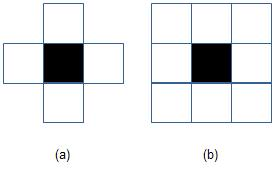
\includegraphics[width=.3\textwidth]{images/neighbourhoods.png}
\caption{(a) von Neumann Neighbourhood and (b) Moore neighbourhood on a 2D square lattice \cite{debasis2011survey}}
\label{fig:neighbourhoods}
\end{figure}

In a finite grid CA, border cells must be given special consideration since they do not have the same number of neighbours as interior cells and therefore cannot share the same neighbourhood function. One option is to define a case-wise neighbourhood function with different behaviour for border cells. Another option is to freeze the state of border cells. In the field of partial differential equations, this is known as setting "fixed boundary conditions".  The problem can also be circumvented entirely by relaxing the finite grid assumption and allowing cells to "wrap around" the grid. This is known as setting "periodic boundary conditions" and can be imagined visually as running the CA on an infinite periodic tiling or, alternatively, on a torus.


\subsection{Life-Like CA} \label{sub:life}
The most popular example of a CA is the Game of Life (henceforth "Life") formulated by John Conway in 1970 \cite{gardner1970fantastic}. It consists of a 2D grid of cells, each with a boolean state variable signifying that the cell is either "alive" or "dead". The transition rule takes as input the cell's own state $\sigma_i(t)$ and the number of living individuals in the cell's Moore neighbourhood (excluding itself), denoted $n_i(t)$. This is as follows:

\begin{equation}
  \phi(\sigma_i(t), n_i(t)) = 
\begin{cases}
  0 & \sigma_i(t) = 1 \text{ and } n_i(t) < 2 \text{  (Death by "exposure")}\\
  0 & \sigma_i(t) = 1 \text{ and } n_i(t) > 3 \text{  (Death by "overcrowding")}\\
  1 & \sigma_i(t) = 1 \text{ and } n_i(t) \in \{2,3\} \text{  (Survival)}\\
  1 & \sigma_i(t) = 0 \text{ and } n_i(t) = 3 \text{  (Resurrection)}\\
  0 & \sigma_i(t) = 0 \text{ and } n_i(t) \neq 3 \\
\end{cases}
\end{equation}

Despite its simple setup and update rule, Life can exhibit the emergence of complex patterns. It is possible to simulate a fully universal Turing machine within Life\cite{rendell} and, as a corollary of the Halting Problem, this means that Life is undecidable. Given two arbitrary configurations, it is impossible to algorithmically determine whether one will follow the other.\\

Patterns found within Life include fixed-point solutions to the transition function like the \textit{block} as well as periodic oscillators like the \textit{beacon} which has period 2. There are also periodic patterns that move across the lattice such as the \textit{glider} pattern. The density of a state is the number of living cells as a ratio of total grid size. It is possible to discover new stable patterns by repeatedly running specific rules on random initial states of a pre-determined density (called soups) and classifying the objects remaining after transient patterns have dissipated. Large-scale experiments of this nature are called "soup searches"\cite{flammenkamp}.\\

\begin{figure}[H]
\centering
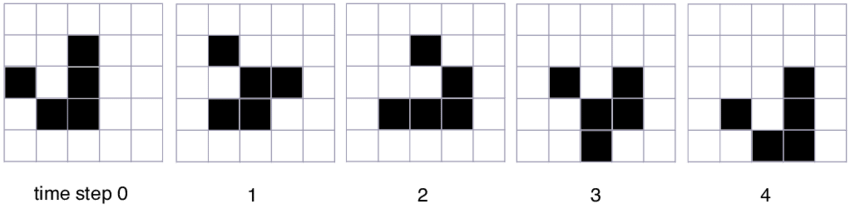
\includegraphics[width=0.8\textwidth]{images/life-glider.png}
\caption{The glider pattern in the Game of Life \cite{dorin2012framework}}
\label{fig:life-glider}
\end{figure}

A CA is considered "Life-like" if it exists on a 2D lattice, has binary state, and uses the Moore neighbourhood function. Life-like CA exist in two varieties: inner-totalistic and outer-totalistic.

\begin{definition}[Inner-Totalistic]
A Life-like CA is inner-totalistic if the output of the transition function depends only on the number of living cells in a cell's neighbourhood (including the cell itself).
\begin{equation}
  \sigma_i(t+1) = \sigma_j(t+1) \iff \sum_{\mathclap{c_p \in \mathcal{N}(c_i)}}\sigma_p(t) = \sum_{\mathclap{c_q \in \mathcal{N}(c_j)}}\sigma_q(t)
\end{equation}
\label{def:inner-totalistic}
\end{definition}

\begin{definition}[Outer-Totalistic]
A Life-like CA is outer-totalistic if the output of the transition function depends on both the number of living cells in a cell's neighbourhood and the state of the cell itself.
\begin{equation}
  \sigma_i(t+1) = \sigma_j(t+1) \iff \sum_{\mathclap{c_p \in \mathcal{N}(c_i)}}\sigma_p(t) = \sum_{\mathclap{c_q \in \mathcal{N}(c_j)}}\sigma_q(t) \quad \textnormal{and} \quad \sigma_i(t) = \sigma_j(t) 
\end{equation}
\label{def:outer-totalistic}
\end{definition}

As an example of the subtle difference here, consider the configurations shown in Figure~\ref{fig:two-moores}. An inner-totalistic CA would yield identical configurations in the next time step since both input configurations have 3 active cells in the neighbourhood set. However, an outer-totalistic CA would treat both configurations differently as one has an live centre cell and the other has a dead centre cell. This discrepancy corresponds to a great difference in the size of search spaces. There are $2^{10}=1024$ inner-totalistic CA but $2^{18} = 262144$ outer-totalistic CA. We represent the transition function of an outer-totalistic CA in a form called birth-survival (B/S) notation. Using this notation, we can represent the Game of Life as B3/S23. In this thesis, when we refer to Life-like CA, we implicitly assume the outer-totalistic variety.\\

\begin{figure}[!h]
  \centering
  \hfill
  \subfloat{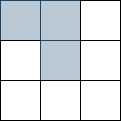
\includegraphics[width=.15\textwidth]{images/moore_1.png}}\hfill
  \subfloat{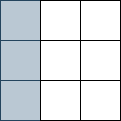
\includegraphics[width=.15\textwidth]{images/moore_2.png}}\hfill\hfill
  \caption{Two possible configurations of a Life-like CA}
  \label{fig:two-moores}
\end{figure}

\begin{definition}[Birth-Survival notation]
Let $N_b$ and $N_s$ be sets of integers. We say an outer-totalistic CA has rulestring \textnormal{B$N_b$/S$N_s$} if it has transition function:
\begin{equation}
  \phi(\sigma_i(t), n_i(t)) = 
  \begin{cases}
    1 & \sigma_i(t) = 0 \text{ and } n_i(t) \in N_b \text{  (Birth)}\\
    1 & \sigma_i(t) = 1 \text{ and } n_i(t) \in N_s \text{  (Survival)}\\
    0 & \text{otherwise}
  \end{cases}
\end{equation}
\label{def:bs-notation}
\end{definition}


\subsection{Elementary CA} 
Elementary CA are defined on the simplest nontrivial lattice, a finite one-dimensional chain. The neighbourhood of each cell contains the cell itself and the two cells adjacent to it on either side. The state variable is a boolean which means there are $2^3 = 8$ possible neighbourhood state configurations. A transition rule maps each of these neighbourhood states to a resultant state and can therefore be represented as an 8-digit binary rule table $(t_7t_6t_5t_4t_3t_2t_1t_0)$ where configuration $(000)$ maps to $t_0$, $(001)$ maps to $t_1$, ..., and $(111)$ maps to $(t_7)$. Consequently, there are $2^8=256$ possible transition functions for elementary CA.\\

The Wolfram code, a number between 0 and 255 obtained by converting the binary rule table to decimal, is the standard naming convention for these rules. Rule 110 is particularly notable as it can exhibit  and is Turing complete \cite{cook2004universality}. Figure \ref{fig:rule-110} shows an example progression of a Rule 110 system. Each row of pixels represents the state of the automaton at one snapshot in time with the topmost row representing the randomized initial state. It shows the emergence, interaction, and subsequent dissipation of multiple long-lived impermanent patterns. This is called class 4 behaviour\cite{wolfram2002} (see Def~\ref{def:wolfram-classes}).

\begin{figure}[!h]
\centering
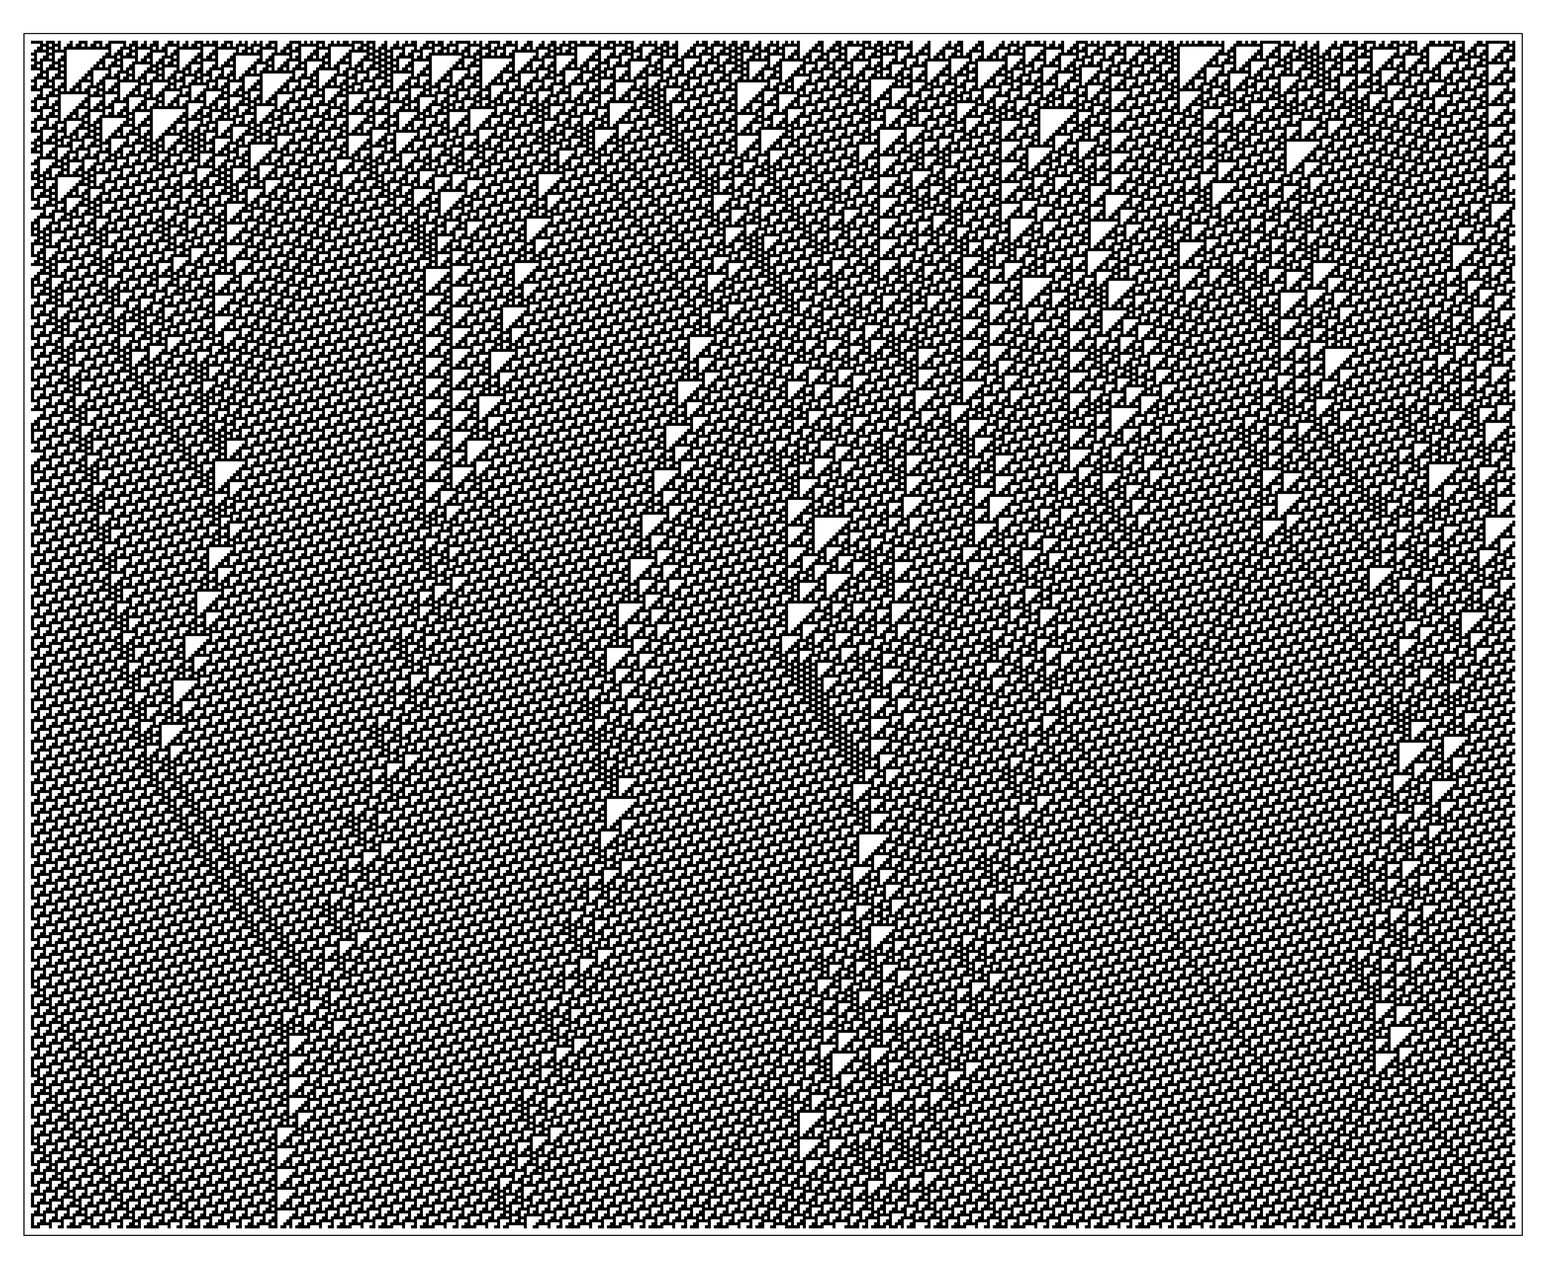
\includegraphics[width=0.65\textwidth]{images/rule-110.png}
\caption{Rule 110 progression with random initialisation \cite{wolfram2002}}
\label{fig:rule-110}
\end{figure}

\section{Turing Patterns}
Morphogenesis is the process by which a system develops into a particular shape or pattern.  Biologically, this is seen in most multicellular organisms which can robustly develop specialised organs and intricate skin patterns without any centralised decision-making. Through simple rules encoded in the genome and homeostatic feedback loops enforced through chemical signalling, a tissue knows exactly how to grow and when to stop.

\begin{figure}[H]
\centering
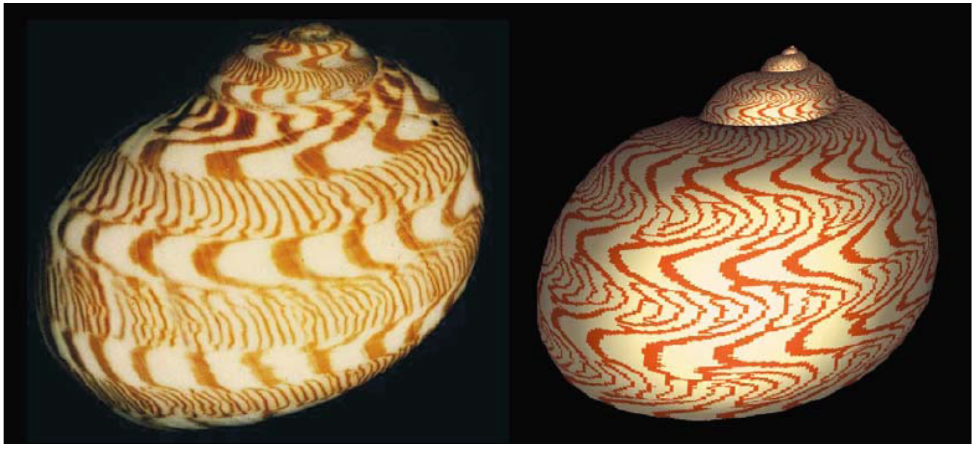
\includegraphics[width=0.6\textwidth]{images/turing-shell.png}
\caption{Complex patterns on sea shells (left) can be replicated using Turing patterns (right) \cite{meinhardt2009algorithmic}}
\label{fig:seashells}
\end{figure}

In \textit{The Chemical Basis for Morphogenesis (Turing, 1952)}\cite{turing1990chemical}, Alan Turing proposes that spatially periodic phenomena in the natural world like the stripes on a zebra or the skin patterns on pufferfish can arise autonomously from random or uniform initial conditions through the interaction for two diffusible substances. These patterns are known as Turing patterns and Turing's model forms the basis of major theories in developmental biology. Such patterns are visible at all scales from the fold patterns of mammalian brains\cite{cartwright2002labyrinthine} to the distribution of matter in the Milky Way\cite{smolin1996galactic}. Figure~\ref{fig:seashells} is an example of Turing patterns on sea shells.

\subsection{Gray-Scott Model}

Turing patterns arise out of two component reaction-diffusion systems. One specific example is the Gray-Scott model\cite{gray1983autocatalytic} in which one component, $U$, is consumed while the other, $V$ is produced in a chemical reaction. In this thesis, we consider a simple reaction scheme called cubic autocatalysis where the following reaction occurs with a certain probability
\begin{equation}\label{eq:gs-main}
  U + 2V \rightarrow 3V
\end{equation}
To compensate for $U$ being consumed, the system replenishes $U$ and removes $V$ by rates controlled with feed and kill factors $f$ and $k$ respectively. The substances diffuse over the grid at rates $r_u$ and $r_v$. The system is characterised by two equations.
\begin{definition}[Reaction-Diffusion System] \label{def:reaction-diffusion}
\begin{align} 
  \label{eq:gs-u} \pdv{u}{t} &= -uv^2 + f(1-u) + r_u \nabla^2 u\\
  \label{eq:gs-v} \pdv{v}{t} &= uv^2 - (f+k)v + r_v \nabla^2 v
\end{align}
\end{definition}
where $u$ and $v$ represent the densities of each component in a given cell. $\pdv{u}{t}$ and $\pdv{v}{t}$ represent the change in these densities with respect to time. Each density has three sources of change described by the three terms on the right hand side of each equation. The first term describes the reaction \ref{eq:gs-main} where one $U$ molecule reacts with two $V$ molecules which is why the term is a product of $u$ and $v^2$. The second term represents external inputs and outputs. In \ref{eq:gs-u}, the feed rate is multiplied by $1-u$ so that replenishment depends on current density. In \ref{eq:gs-v}, $v$ is multiplied by $-(f+k)$ so that $V$ is removed faster than $U$ is added. Finally, the third term describes the change in each density due to diffusion using the 2D Laplacian to get the difference between a cell's current state and the average of the neighbourhood cell states.\\

For most values of feed and kill rate, the Gray-Scott model attains one of two quiescent states, either completely dominated by $U$ or completely dominated $V$. However, there are certain feed and kill rates which elicit complex stable patterns. Many of these bear a strong resemblance to Turing patterns observed in nature as shown by Figure~\ref{fig:gs-turing-patterns}.

\begin{figure}[H]
\centering
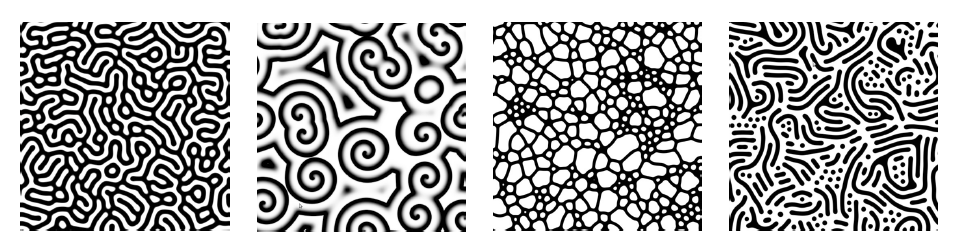
\includegraphics[width=\textwidth]{images/turing-patterns.png}
\caption{Turing patterns arising out of Grey-Scott model simulations\cite{sims}}
\label{fig:gs-turing-patterns}
\end{figure}

\section{Evolutionary Algorithms}

Evolutionary algorithms (EAs) are a family of heuristic-based search algorithms for black-box optimisation problems. They are inspired by biological evolution. A chromosome is an indirect encoding of a candidate solution. The structure of the chromosome is called the "genotype" and the behaviour of the corresponding candidate solution is called the "phenotype". The fitness of a candidate is calculated from its phenotype. An evolutionary algorithm initializes population of chromosomes and modified them through repeated recombination, mutation, and selection. The purpose of recombination is to produce new solutions with "fit" attributes by combining aspects of existing candidates. Mutation, on the other hand, is applied to explore new areas of the search space by randomly perturbing existing candidates. Mutations may lead to weaker candidates in the short term but is useful as a method of discovering new attributes that, over many generations, can produce fitter candidates. Finally, selection applies competitive pressure to the population, ensuring that the overall fitness of the population is improving and increasingly fit solutions are being discovered.\\

EAs are valued for their broad applicability as they require no information about the constraints or derivative of the objective function. In fact, an explicit representation of the objective function is not even neccessary to run an EA as long as candidates can be compared to each other. Selection pressure can then be introduced in the form of tournament-based elimination.

\subsection{Genetic Algorithms}

A genetic algorithm (GA) is a particular type of evolutionary algorithm with binary string genotype. For a genetic algorithm, we perform recombination by randomly picking two parents with replacement from the elite subset and mixing their chromosomes to produce a child. This is called crossover. We formalise the structure of a genetic algorithm in Algorithm~\ref{alg:ga}.\\

\begin{algorithm}
  \caption{Schematic Genetic Algorithm}\label{alg:ga}
  \begin{algorithmic}
  \Require $S$ - the set of possible chromosome values
  \Ensure $s^* \in S$
  \State $t \gets 0$
  \State $M_0 \gets \mu$ random individuals from $S$
  \While{stopping condition is false}
    \State \Call{Evaluate}{$M_t$}
    \State $P_t \gets$ \Call{SelectParents}{$M_t$}    \Comment{Parents}
    \State $\Lambda_t \gets$ \Call{Recombine}{$P_t$}  \Comment{Children}
    \State $Pmod_t \gets$ \Call{Mutate}{$P_t$}
    \State $\Lambda mod_t \gets$ \Call{Mutate}{$\Lambda_t$}
    \State $M_{t+1} \gets$ \Call{SelectPopulation}{$Pmod_t$, $\Lambda mod_t$}
    \State $t \gets t+1$
  \EndWhile
  \State $s^* \gets$ \Call{FindBestCandidate}{$P_t$}
  \end{algorithmic}
\end{algorithm}

The initial selection phase ($\Call{SelectParents}$) uses a fitness function to compare and select the top candidates. The latter selection phase ($\Call{SelectPopulation}$) produces a new population from the modified parents and children. Population-wide selection criteria can be enforced in this phase. For example, weak parents can be eliminated if they have survived for too many generations or, symmetrically, children can be granted immunity for a particular number of generations.\\

Genetic operators are specific implementations of actions such as crossover and mutation. The most common mutation operator is pointwise mutation where each bit in the chromosome is flipped with some fixed probability $p$. The three common crossover operators used in genetic algorithms are:
\begin{enumerate}
  \item Uniform Crossover: For each bit (or "gene") in the chromosome, copy the corresponding gene from one parent.
  \item Single Point Crossover: Randomly pick a split point. Take the all bits to the left of the split point from one parent and all bits to the right from the other.
  \item Multiple Point Crossover: Randomly pick $n$ split points. Alternate picking contiguous sections of the chromosome between split points from each parent.
\end{enumerate}

% \begin{figure}[!h]
% \centering
%     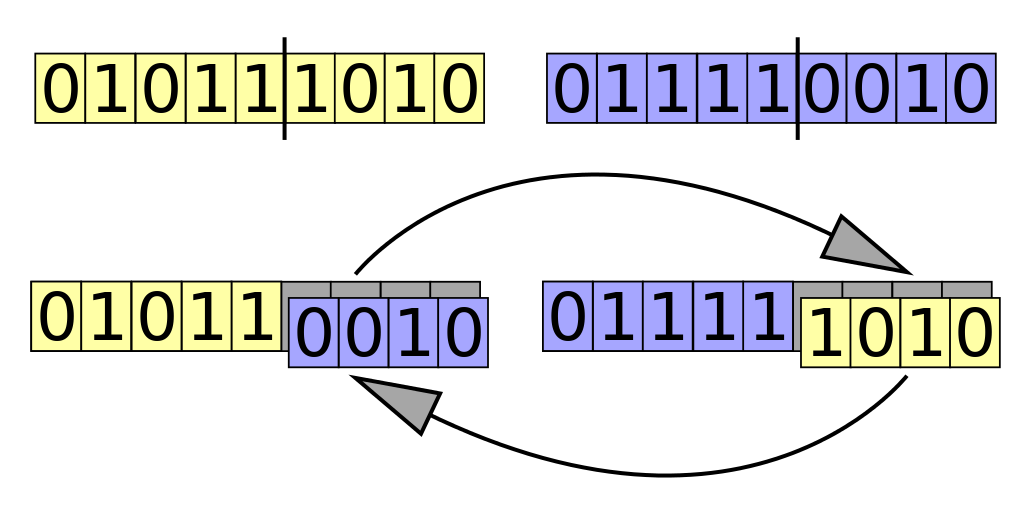
\includegraphics[width=.5\textwidth]{images/single-crossover.png}
%     \caption{Visualisation of single-point crossover on 9-bit chromosomes. \cite{singlecrossover}}
% \label{fig:single-crossover}
% \end{figure}

